
%%%%%%%%%%%%%%%%%%%%%%% file typeinst.tex %%%%%%%%%%%%%%%%%%%%%%%%%
%
% This is the LaTeX source for the instructions to authors using
% the LaTeX document class 'llncs.cls' for contributions to
% the Lecture Notes in Computer Sciences series.
% http://www.springer.com/lncs       Springer Heidelberg 2006/05/04
%
% It may be used as a template for your own input - copy it
% to a new file with a new name and use it as the basis
% for your article.
%
% NB: the document class 'llncs' has its own and detailed documentation, see
% ftp://ftp.springer.de/data/pubftp/pub/tex/latex/llncs/latex2e/llncsdoc.pdf
%
%%%%%%%%%%%%%%%%%%%%%%%%%%%%%%%%%%%%%%%%%%%%%%%%%%%%%%%%%%%%%%%%%%%


\documentclass[runningheads,a4paper]{llncs}

\usepackage{amssymb}
\setcounter{tocdepth}{3}
\usepackage{graphicx}
\usepackage{lscape}
\usepackage{url}
\usepackage{subfigure}
\urldef{\mailsa}\path|{wendpanga-francis.ouedraogo,frederique.biennier}@liris.cnrs.fr|
\urldef{\mailsb}\path|{philippe.merle}@inria.fr|    
\newcommand{\keywords}[1]{\par\addvspace\baselineskip
\noindent\keywordname\enspace\ignorespaces#1}

\begin{document}

\mainmatter  % start of an individual contribution

% first the title is needed
\title{Contextualised security operation deployment through MDS@Runtime architecture}

% a short form should be given in case it is too long for the running head
\titlerunning{Lecture Notes in Computer Science: Authors' Instructions}

% the name(s) of the author(s) follow(s) next
%
% NB: Chinese authors should write their first names(s) in front of
% their surnames. This ensures that the names appear correctly in
% the running heads and the author index.
%
\author{Wendpanga Francis Ouedraogo%
\thanks{Please note that the LNCS Editorial assumes that all authors have used
the western naming convention, with given names preceding surnames.}%
\and Fr\'ed\'erique Biennier \and Philippe Merle}
%
\authorrunning{Gestion Contextualis\'ee de la S\'ecurit\'e}
% (feature abused for this document to repeat the title also on left hand pages)

% the affiliations are given next; don't give your e-mail address
% unless you accept that it will be published
\institute{Universit\'e de Lyon, CNRS INSA-Lyon, LIRIS UMR 5205, 20 avenue Albert Einstein, 69621 Villeurbanne Cedex, France\\
Inria Lille - Nord Europe, Parc Scientifique de la Haute Borne, 40 avenue Halley, 59650 Villeneuve d'Ascq, France\\
\mailsa\\
\mailsb\\}

%
% NB: a more complex sample for affiliations and the mapping to the
% corresponding authors can be found in the file "llncs.dem"
% (search for the string "\mainmatter" where a contribution starts).
% "llncs.dem" accompanies the document class "llncs.cls".
%

\toctitle{Lecture Notes in Computer Science}
\tocauthor{Authors' Instructions}
\maketitle

\begin{abstract}
The development of collaborative business leads to new challenges for corporate information systems such as interoperability, elastic deployment and security management in dynamic contexts. To fit these challenges one can take advantage of the agility and elasticity provided by Service Oriented Computing and Cloud Computing. To support an adaptive and contextualised security deployment providing a consistent protection level despite the changing contexts, we propose MDS@run.time the marriage of both Model Driven Security and Model@run.time approaches. Security policy models (produced by a MDS process) are interpreted at run.time depending on the context (Model@run.time). To this end we propose an architecture that can be plugged on any hosting middleware to manage the security mediation (i.e. select, compose and orchestrate security services) depending on the protection requirements defined in the security policy. A Security as a Service component is also proposed to support this "security outsourcing" strategy. This proposition is illustrated thanks to a Proof of Concept prototype built on top of the FraSCAti middleware.
\end{abstract}

\section{Introduction}
The development of Collaborative Business strategies leads to reorganize the corporate information system deployment in order to increase its agility. Taking advantage of the agility and interoperability of SOA, collaborative Business Process can efficiently be built by composing business services depending on business needs. Nevertheless, such collaborative organization challenges contextualized security deployment as a same business service may be used in different collaborative context and orchestrated using different runtime environment.
To fit this challenge, we've proposed to extend the Model Driven security approach to capture information and services protection requirements using an “end user oriented” set of questions to capture the patrimonial importance of these elements so that confidentiality, availability, integrity requirements can be consistently defined and used to annotate the Business Process specification. Then we use a model driven generation process to define the security policies associated to the services implementing the collaborative Business Process.
These security policies are seen as an abstract Model@Runtime protection specification. Depending on the runtime environment different security services must be selected and orchestrated to fulfill the protection requirements. To this end, we propose a SecurityModel@Runtime component that intercepts the service invocation, extracts its security policy and orchestrates the required protection services depending on the execution environment before launching the “functional” service. 
After presenting briefly the context and state of the art limits, we detail our SecurityModel@Runtime, paying attention on the way it can be plugged on the service execution middleware before showing the impact on the execution performances due to the policy interpretation.

\section{From MDS to MDS@Runtime}
\label{mdsToMds@Runtime}
The increased importance of Collaborative Business strategies leads to reorganize the corporate information system deployment in order to increase its agility and interoperability so that common Business Process supporting these collaborative organisation can be efficiently designed and deployed. Taking advantage of the agility and interoperability of SOA and Cloud environments, such collaborative Business Process can be built by composing business services before deploying them on cloud platforms depending on the needs. This leads to a "de-perimetrised" information system organization, as business services can be selected,  composed and orchestrated in various contexts, challenging a consistent and contextualised Business service protection.
For example (Fig~\ref{fig:bp}), setting a e-government service to improuve a scholarship management process
 lead to the development of a collaborative "on-line" e-governement organisation allowing both students, grant administration and academic partners to share students curriculum information. To this end, a common Business Process associated to scholarship business feature is built, combining services and personal workflows from both grant adaministration and academic partners, challenging new security features such as partner authentication, access control on the student information non repudiation...  

\begin{figure}  
\centering
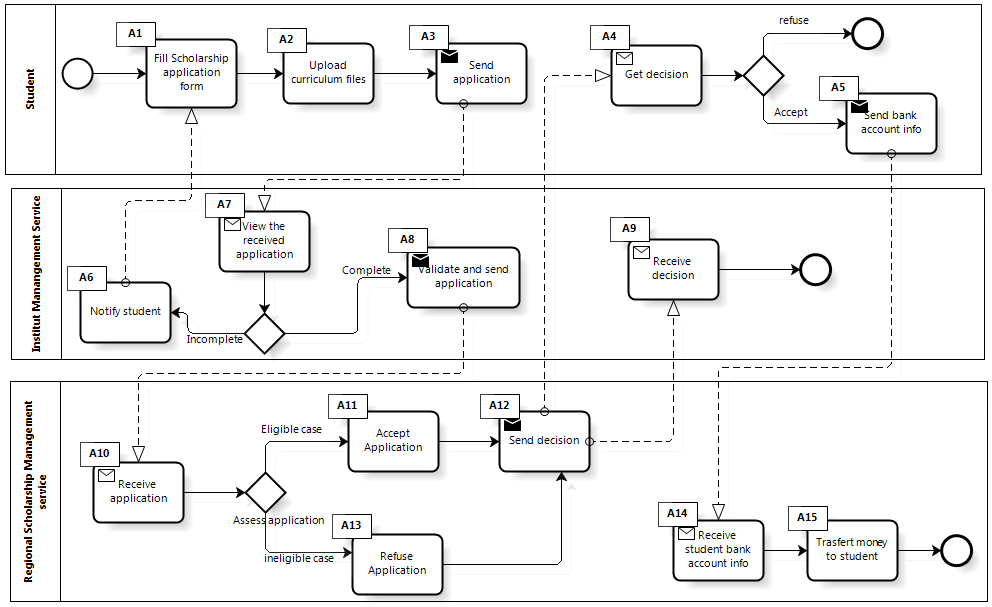
\includegraphics[height=200pt, width=320pt]{BRPE_Eng1.png}
\caption[Scholarship management process]{Scholarship management process\\ To illustrate our approach, we propose to use a process of the scholarship award by the region, which collaborate with the institut in a e-government logique. In this example, each student fill a scholarship application form, upload various documents (resume, cover letter, diplomas, ...) and submit its request. Then, the institute manager, view and check each student application data to ensure that it is compliant before sends it to the region. At the regional level, applications are analyzed by agents, who decide to award or not scholarships based on eligibility criteria. Once the decision is taken by these agents, a notification is sent to each student and each school principal is informed about the decision. Students whose applications have been accepted are then requested to send their bank account information to the region in order to trasfert scholarship money.
In this esxemple, the student application contains personnal data which require to be protected. For that, we have to secure these data against the unauthorized access.  }
\label{fig:bp}
\end{figure}


We propose to focus on the student data activity access. 
we propose a simple use case to control access to the student data. During our approach based MDS patterns implementation, security policies are automatically generated (see Fig.~\ref{fig:policy}) and associated to "Scholarship" service (see Fig.~\ref{fig:wsdl}).

\subsection{Securing services}
Depending on the perceived security risks / system vulnerabilities, different security requirements can be set. Based on the ISO/IEC 27002, the OASIS Service Reference Model (~\cite{OAS06}) defines different security requirements (Condidentiality and privacy management, Integrity, Authentication, Authorisation, Availability and Non Repudiation) that  requires the deployment of security means from the network layer (which is rather focused on the availability requirement and protection against deny of service attacks)and transport layer (which has to provide secured confidential channel between tranmitters and receivers) to the Application layer which manages most of the security requirements (Authentication, Authorisation, Non repudiation, confidentiality and privacy...). Different standards such as WS-Security, SAML, XACML, BSLA...(see XX FIG ou tableau XX) have been developped to support these security requirements implementation.
Such protection means can either be deployed directlty in the service operation or "attached" to the service interface specification. To this end, Security policies can be used to specify the required protection levels and means to be deployed, allowing an easier "upgrading" of protection requirement. 
For example, authenticating students and or academic partners, building secured communication channels and establishing non repudiation features could be achieved by combining different protection means (see the secvurity policy that could be attached to the service) (Fig~\ref{fig:policy}). By this way, service operations are not affected while security requirements are taken into account.

\begin{figure}  
\centering
\includegraphics[height=135pt, width=380pt]{scholarshipPolicies.png}
\caption{Security policies associated to « Scholarship » resource.}
\label{fig:policy}
\end{figure}
These policies specify that the service has an operation named "ViewStudentData", which is considered as a resource (line 2 in Fig.~\ref{fig:policy}). This resource requires authentication (lines 2-8) by login /password (line 4) with the reference to the user authentication checking file specified on line 5. Besides authentication, access control (lines 9-16) using ACL (line 12), with time constraints (line 10) should be applied to this resource. Fig.~\ref{fig:acl} describes the contents of the  autorization file. It shows that users can access the resource at specific hours (between 6am and 12pm for user "user1").
 
 
\begin{figure}
\centering
\includegraphics[height=55pt, width=380pt]{scholarshipAcl.png}
\caption{Authorization file « AccessControlList.xml ».}
\label{fig:acl}
\end{figure}


\subsection{MDS for Services}

Different methods can be used to set a consistent security policy, based on vulnerability and threats models as EBIOS, MEHARI, OCTAVE, SNA... However, they are complex and designed for a perimetrised environment and are not "end-user" oriented. To overcome these limits, business architects should be able to define security policies while building new business process. To this end, Model Driven Security can be used to attach security requirements specification in the Business Process and generate adapted security policies. In previous work, we have proposed in ~\cite{OBG12} to enrich the MDS approach with a security pattern engineering strategy to capture protection requirements and deployment platform information to generate automatically the security policies that will be attached to the different services (see Fig~\ref{fig:mds}).

\begin{figure}  

\centering
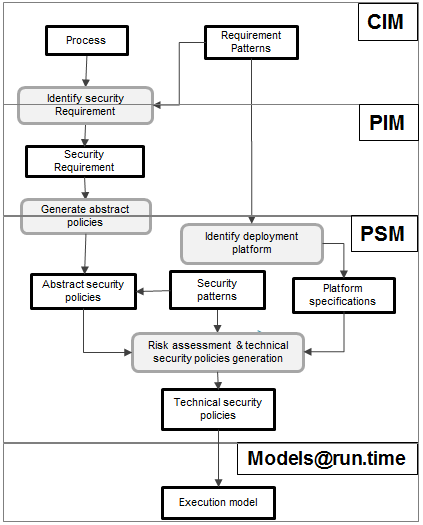
\includegraphics[height=200pt, width=160pt]{mds.png}
\caption{Security policy generation process based on MDS}
\label{fig:mds}
\end{figure}

These security policies, which are in fact our security model at runtime, are associated with the service description (see Fig.~\ref{fig:wsdl}), including the reference to the policy file (line 3). This allows during business service execution to identify the security policies to be applied.
\begin{figure}  
\centering
\includegraphics[height=120pt, width=380pt]{scholarshipWSDL.png}
\caption{Link policy file with operation \emph{«ViewStudentData»} of the \emph{«Scholarship»} service WSDL.}
\label{fig:wsdl}
\end{figure}

\begin{figure}  
\center
\includegraphics[height=105pt,width=380pt]{scholarshipComposite.png}
\caption{Link \emph{Scholarship} component with \textbf{MDS@Runtime} component.}
\label{fig:gestionEtudiant}
\end{figure}

In our example,the student curriculum activity and the related information must be protected in the new "openned" context. This confidentiality requirement impacts both application layer which will be in charge of the access control (i.e. authentication and authorisation management) and the transport layer (Fig~\ref{fig:policy}). 
To provide a consistent protection of the information system, the security policies must be used to compose and orchestrate security services accordingly. Taking into account more precise information on the execution context could improve both the service operation performance and the protection level, avoiding under / over protection deployment. In our example, each employee of the academic partners can accede to the curriculum activity from the already secured partner network. Once the security policy is attached to the collaborative workflow, access control including a systematic authentication is required to fulfill the non repudiation requirement as well as log features and network encryption, despite the secured access provided by the corporate infrastructure (namely authentication to unlock the workstation and secured infrastructure). (Table ~\ref{tab:tab1}) shows a comparison of service execution time with / without authentication and authorization.
\begin{table}

\caption{Services execution time}
\begin{tabular}{@{}*{2}{|p{5cm}}|}
\hline
Executed component & Run time execution(ms)\\
  \hline
 Business service & 59\\
 Business service \& Authentication & 69\\ 
 Business service \& Authentication \& Autorization & 72\\ 

    \hline
\end{tabular}
\label{tab:tab1}
\end{table}
To avoid this costly over-protection or risky under-protection depending on the runtime environment vulnerability, we propose to turn these security policies as Model@runtime so that they can be analysed to select, compose and orchestgrate the most convenient security services depending on the exact runtime environement. This requires a new architecture to "outsource" the security management as a new high-level service that can be plugged on the execution middleware. In the next section, we'll present this new architecture and a proof of concept based on the Frascati middleware.


\subsection{MDS@Runtime: Adapting security deployment in service operation}

Implementing a Service Oriented Architecture (SOA) requires a middleware for both integration and distributed communication. Middleware plays an intermediary role between the client and the service provider. It is a software component which is located between the operating system and business applications and offers an abstraction high level for building distributed applications. It allows business services integration and management, and provides access to various external services ~\cite{SHLP05}. It is an integration solution which implements a fully distributed architecture (deployment on multiple nodes), providing services such as data processing or routing based on the content (CBR), and a higher level of interoperability by use systematically standards such as XML, Web Services specifications and WS-* ~\cite{Lou08}.
 

Our architecture is built on the traditional service / middleware / hosting platforms architecture (see fig X.a). In order to avoid under or over protection depending on the runtime context, we propose to outsource the security management. As stated in the previous section, the security policy attached to the different business services expresses the protection requirement for this service. Plugged on the classical business service / middleware / hosting cloud platform(s) architecture, our MDS@Runtime environment (see fig XX) consists in :

\begin{itemize}
\settowidth{\leftmargin}{{\Large$\square$}}\advance\leftmargin\labelsep
\itemsep5pt\relax
\renewcommand\labelitemi{{\lower1.5pt\hbox{\Large$\square$}}}
\item A specific Interceptor component plugged on the middleware intercepts the service /middleware interaction (step 1) and routes this interaction to the MDS@Runtime component (step 2) 
\item	The MDS@runtime component  is the core component to acheive the dynamic security deployent. It consists in a 3 sub components : 
\begin{itemize}
\item	The policy manager parses the service description, extracts and loads the associated policy files before launching the conrtext acquisitopn process.
\item The context manager collects information associated to the execution context (steps 3 and 4). It transfers the results to the security mediator
\item	The security mediator parses the security policy to get the protection level associated to each security service. Depending on the execution context, it selects and composes security services to implement the required protection. Then it orchestrates the security services invocation (steps 5 and 6) and if it succeedes it routes back the business service / middleware interaction to the middleware.
\end{itemize}
\item The Security as a Service (IV) component gathers implementation of various security services (authentication, autorisation, integrity controls…) in a SaaS vision.
\end{itemize}
\begin{figure}
    \centering
    \subfigure[Multilayer architecture]{\label{sub1} 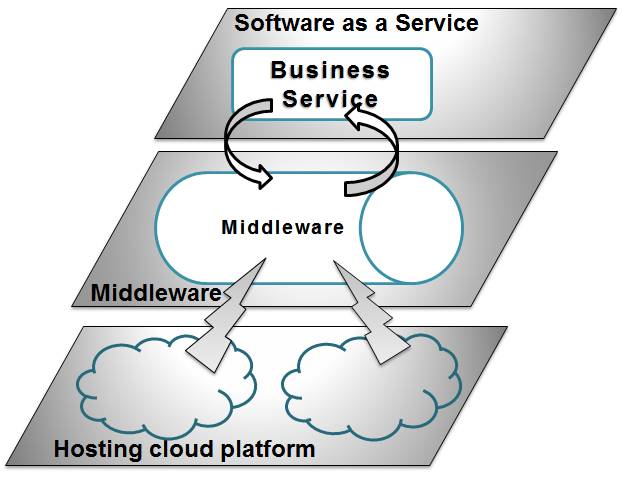
\includegraphics[height=120pt, width=120pt]{architecture2.PNG}}
    \subfigure[Multilayer architecture with MDS@Runtime]{\label{sub2} 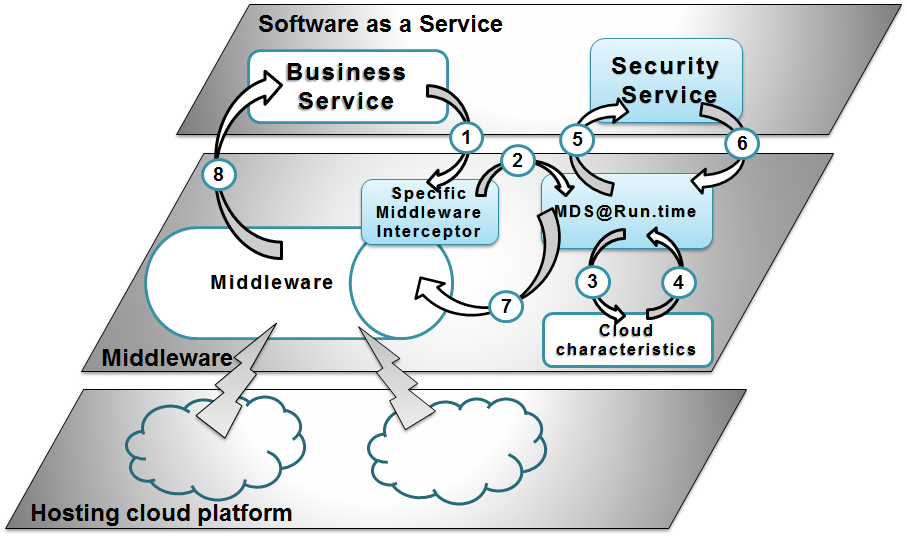
\includegraphics[height=180pt, width=215pt]{architecture1.PNG}}
    \caption{MDS@Runtime architecture}
    \label{fig :archi}
\end{figure}

\section{Implementation : MDS@Runtime with FraSCAti}


FraSCAti ~\footnote{\url{http://frascati.ow2.org}}~\cite{SMF09}~\cite{SMR12} is a middleware based on the OASIS Service Component Architecture (SCA) standard to build service-oriented and adaptable business applications. FraSCAti applications can be deployed in different clouds (Amazon EC2 , Amazon Elastic BeanTalk , Google App Engine, CloudBees , etc.)~\cite{MRS11}~\cite{PHM12}. The adaptability at the design is based on the fact FraSCAti platform was designed as a plugin-based architecture to adapt to different execution environments and to select on demand, the required application functionality to compose its platform. The adaptation to the execution is based on FraSCAti reflective features, which mean the capacity for applications introspection and reconfiguration at runtime. [motive choix pour le POC on detaille la mise en oeuvre]

FraSCAti provides a framework for programming, deploy and execute components achieving as services which are OASIS SCA standard compliant. To ensure the business processes security deployed on cloud infrastructures, we pro- pose a security framework based on SCA components which can be plugged to FraSCAti platform. 

\begin{figure}[ht]  
\centering
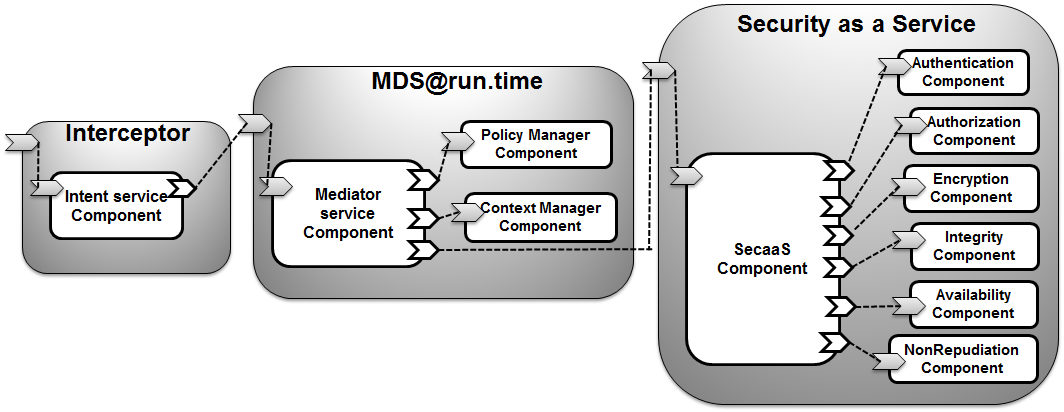
\includegraphics[height=150pt, width=350pt]{composites2.png}
\caption{Security composites.}
\label{fig:compoites}
\end{figure}


\subsection{FraSCAti Intent for MDS@Runtime}
 The \emph{Intent} component is responsible for detecting and intercepting business services invoked  by clients. This component uses the aspect-oriented programming (AOP) techniques implemented in FraSCAti to perform actions before, during and after each business services invocation. These techniques use the Apache CXF interception mechanisms embedded in FraSCAti. 
   The \emph{Request} component plays the intermediary role between FraSCAti middleware and security services. It provides a bidirectional interface that allows the component Intent to formalize the interaction messages received from the FraSCAti platform and also to specify orders toward the FraSCAti platform which performs some technical actions. This component ensures a total independence between the FraSCAti middleware and our security system, allowing one hand, the security services,  to be able to deploy and run on any other middleware and second hand, to deploy on a specific platform just the required security services.


The composite MDS@Runtime  (see Fig~\ref{fig:mdsAtRuntime}) is invoked by the intent component of the interceptor composite. Il includes:


\begin{itemize}
\settowidth{\leftmargin}{{\Large$\square$}}\advance\leftmargin\labelsep
\itemsep8pt\relax
\renewcommand\labelitemi{{\lower1.5pt\hbox{\Large$\square$}}}

\item The \emph{Mediator} component is responsible for analyzing called service requests intercepted by the  \emph{Intent} component and  encapsulated by the \emph{Request} component. It also identify the security policies rules associated to business service with which the client needs to interact. Thus, through the \emph{Request} component, the \emph{Mediator} receives information of the services involved in the interaction. This information is used to get policies associated to resources (the business services functionality implemented by service operation). These policies are then analyzed and orchestrated by the \emph{Mediator} to call the required security services.
\item The \emph{PolicyManager} component manages the policies. It receives from the \emph{Mediator} the resource or service reference requested and the policy file link. It returns to the \emph{Mediator} the list of policies to apply.
\item The \emph{ContextManager} component analyses security policies associated to services and identifies the different policies to be applied according to the user context, the execution environment and security policies associated to the client and service provider. It also provides to the \emph{Mediator} component information such as policies and policies rules related to the execution context. These policy rules are used by the \emph{Mediator} component to call the technical security services.
\end{itemize}


\subsection{Composite SecaaS}

The \textbf{Security as a Service} composite is invoked by the service mediator. It includes various security services which allow protecting resources and business services according to security "as a service" approach. This composite contains the following components (see Fig.~\ref{fig:SecaaS}):


\begin{itemize}
\settowidth{\leftmargin}{{\Large$\square$}}\advance\leftmargin\labelsep
\itemsep8pt\relax
\renewcommand\labelitemi{{\lower1.5pt\hbox{\Large$\square$}}}

\item The \emph{SecaaS} component is the composite entry point. It receives from \emph{Mediator} component, the security policies to be applied. It is responsible for analyzing these policies, to identify the type of security services (authentication, authorization , etc. . ) to call.
\item The \emph{Authentication} component is used to prove the user identity  ( of human or other service). This component receives from SecaaS component, the policy rule to apply, extract information about the security pattern and invokes the security mechanism to be applied. It can be a weak authentication mechanism such as login / password or Strong Authentication such as One Time Password (OTP) or two factors authentication. This authentication component includes subcomponents such as \emph{SSORegistry} ( SSO Single Sign On) component used to store information about sessions authentication  and allow to retrieve user information without restarting authentication.

\item The \emph{Authorization} component allows managing access to resource or service and allows grant or deny the user access to the service. As the authentication , it receives the security policy rule and invokes the authorization mecanism to be applied. This mecanism can be  based on a authorization by role (RBAC) implemented by XACML authorization protocol or a simple Access Control List ( ACL).
\item The Encryption component provides data and messages encryption and decryption mechanism. It also provides secure protocols using  to secure communication (SSL).
\item The \emph{Integrity} component ensures the data and messages integrity exchanged by using messages signature or hash functions.
\item The \emph{Nonrepudiation} component is responsible for recording user actions (authentication, access to data or service, data modification / destruction, etc . ). This information can then be used for auditing and monitoring.
\item The \emph{Availability} component is responsible for the services availability providing access to the service or a clone (redundant service) thereof if the original target service is unavailable. This component also provides backup mechanism to restore system data and services after disaster.


\end{itemize}

The Encryption, Integrity and nonRepudiation components can use security protocols such as WS-Security XML Encryption and XML Signature which provide encryption and signing  exchanged messages mechanisms.


\section{Evaluation}

\label{sec:exemple}

Our performance evaluation is based on the use case prsented section \ref{mdsToMds@Runtime}, focusing on the "ViewStudentData" operation. This operation is implemented thanks to a service associated to a security policy including 
In order to enforce these security policies, the "Scholarship"  Web Service binding (line 6 Fig. ~\ref{fig:gestionEtudiant}) requires to be associated to the \textbf{MDS@Runtime}\footnote{The XML \emph{requires} attribute is the mean for FraSCAti to weave an aspect on SCA component.} composite. This specification allows to intercept calls of the service and invoke the  MDS@Runtime composite before invoking the business service itself.



\begin{figure}  
\center
\includegraphics[height=150pt,width=350pt]{seqGestionEtudiant1.png}
\caption{Interactions inside  \textbf{MDS@Runtime} composite.}
\label{fig:sequence}
\end{figure}


Thank to FraSCAti Explorer tool ~\cite{SMF09}, it is possible, as shown in Fig. ~\ref{fig:sequence}, to follow the invocation of  \textbf{MDS@Runtime} composite components as a UML sequence diagram.


\begin{table}

\caption{Components execution times}
\begin{tabular}{@{}*{3}{|p{3.1cm}}|@{} }
\hline
Component & Run time execution(ms)   & Rate of run time \\[0.2cm]
  \hline
  FraSCAti \& CXF \& Business service & 59&  76\%\\
 FraSCAti Interceptor & 2&  3\%\\ 
 MDS@Runtime & 4&  5\%\\
 Authentication& 10& 13\%\\
 Autorization & 3& 4\%\\
 \hline
   Total & 78& 100\%\\
    \hline

\end{tabular}
\end{table}


\begin{figure}[ht]  
\centering
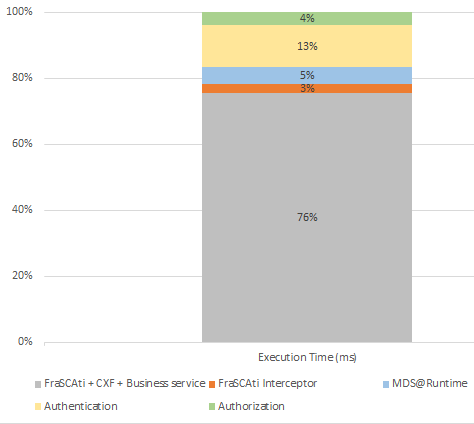
\includegraphics[height=220pt, width=250pt]{runtimeAssessment1.PNG}
\caption{\textbf{Runtime assessment according to the involved components
}}
\label{fig:RuntimeAssess}
\end{figure}








\section{Related works}

Different strategies can be used to provide a consistent protection on Distributed Information Systems, paying attention on both organisational and infrastructure related risks. On one hand, « Security by Design » approaches integrate protection requirements while designing the information system. To this end, different frameworks have been defined to manage security annotations on UML diagrams (such as the multi-purpose UMLSec ~\cite{JJ02} or the rather access control oriented  Secure UML ~\cite{LBD02} Domain Specific languages) or BPMN diagrams (such as ~\cite{WMS09} ~\cite{SSL09}). Taking advantage of such high-level specification specification, the Model Driven Security (MDS for short)  ~\cite{LS09} ~\cite{LZN14} adapts the MDA approach to the security field. Several studies have focused on the use of the MDS approach to secure business process and led to frameworks definition like OpenPMF (XX), SECTET ~\cite{AHB08} and BPSec ~\cite{RFP07}. Nevertheless, none of them support the full transformation process : while BPSec is focused on the requirement engineering part (it includes CIM and PIM models), SECTET and Open PMF provide PIM, PSM and code generation features. Moreover, the generation process is achieved according to a « static » environment vision, i.e. they do not allow any adaptation depending on the execution context. This can lead to under or over-protection depending on the real vulnerabilities / risks associated to the execution platform. Such static infrastructure vision also does not fit the scalable and elastic deployment provided by cloud environments.
On the other hand, Platform Dependent Protection works have been conducted to organise a consistent protection level on cloud based infrastructure such as CSA protection stack or XXX whereas monitoring systems (such as intrusion Detection System XX, vulnerabilities checking XX) are used integrate information on the execution context  and tuen the protection means accordingly. Nevertheless, these works are focused on a « hosting platform protection» vision and do not integrate an « end to end » protection vision. To this end, the the security stack defined in the  OASIS Service reference model defines the way protection requirements should be implemented in a multi-layer architecture (application / Middleware-Transport / network) to improve the global protection consistency while deploying security features associated to a standardised security policy. Nevertheless, this coarse-grain model does not integrate any governance loop so that the execution context can be taken into account while deploying the required protection, leading to either over or under-protection.
To overcome this limit, our MDS@Runtime solution takes advantage of the OASIS security model and of the MDS approach to generate security policies depending on the collaborative BP organisational context (~\cite{OFG13}) so that services can be secured « on demand ». Moreover, it provides a fullt oursourced security environment that can be plugged on the service middleware. Thanks to the execution platform information, collected by the Security Mediator component, security services are selected, composed and orchestrated in a transparent and consistent way, avoiding the costly over protection and the risky under-protection.




\section{Conclusion}
Securing Collaborative Business Process deployed on Cloud systems requires paying attention on both organisational and platform-related vulnerabilities. Taking advantage of the intrinsic flexibility provided by the association of security policies to services, we propose to adapt and extend the MDS strategy to generate security policies and deploying them depending to the execution context. To this end, a MDS@Runtime component is plugged on the middleware, paying attention on the hosting platform models , to select, compose and orchestrate the security services depending on the required protection level depending on the execution context.  The experiment reported in this paper shows how our MDS@runtime architecture can be plugged on the middleware and evaluate its performance level.
Further works will focus on the integration of more detailed platform models and on vulnerabilities monitoring loops so that our coarse-grained vision of the execution context will be refined to ncrease the protection efficiency.






\begin{thebibliography}{4}

\bibitem{BDL03} D. Basin, J. Doser, and T. Lodderstedt. Model Driven Security for Process
Oriented Systems. In 8th ACM Symposium on Access Control Models and
Technologies (SACMAT 03), pages 100–109. ACM, 2003.
\bibitem{CSB08}M. Clavel, V. Silva, C. Braga, and M. Egea. Model-Driven Security in Practice : An Industrial Experience. In 4th European Conference on Model Driven
Architecture : Foundations and Applications (CMDA-FA 08), pages 326–337,
2008.
\bibitem{Lou08} A. Louis. Bus de Service ESB, Nouvelle technologie pour l’int\'egration. Livre
blanc, Petals Link, 2008.
\bibitem{LS09} U. Lang and R. Schreiner. Model Driven Security Management : Making
Security Management Manageable in Complex Distributed Systems. In Workshop on Modeling Security (MODSEC08) - International Conference on Model
Driven Engineering Languages and Systems (MODELS), 2009.
\bibitem{MRS11} P. Merle, R. Rouvoy, and L. Seinturier. A Reflective Platform for Highly Adaptive Multi-Cloud Systems. In International Workshop
on Adaptive and Reflective Middleware (ARM’11) - 12th ACM/IFIP/USENIX
International Middleware Conference, pages 14–21. ACM, 2011.
\bibitem{OBG12} W. F. Ouedraogo, F. Biennier, and P. Ghodous.
Adaptive Security Policy Model to Deploy Business Process in Cloud Infrastructure. In 2nd International Conference on Cloud Computing and Services Science (CLOSER 2012), pages 287–290, 2012.
\bibitem{PHM12} Fawaz Paraiso, Nicolas Haderer, Philippe Merle, Romain Rouvoy, and Lionel
Seinturier. A Federated Multi-Cloud PaaS Infrastructure. In 5th International
Conference on Cloud Computing (CLOUD’12), pages 392–399. IEEE, 2012.
\bibitem{SHLP05} M.-T. Schmidt, B. Hutchison, P. Lambros, and R. Phippen. The Enterprise
Service Bus : Making Service Oriented Architecture Real. IBM Systems Journal, 44 :781–797, 2005.
\bibitem{SMF09}Lionel Seinturier, Philippe Merle, Damien Fournier, Nicolas Dolet, Valerio
Schiavoni, and Jean-Bernard Stefani. Reconfigurable SCA applications with
the FraSCAti Platform. In IEEE International Conference on Services Computing (SCC’09), pages 268–275. IEEE, 2009.
\bibitem{SMR12}L. Seinturier, P. Merle, R. Rouvoy, D. Romero, V. Schiavoni, and J.B. Stefani. A component-based middleware platform for reconfigurable service-oriented architectures. Software : Practice and Experience, 42(5) :559–583, 2012.

\bibitem{SSL09}A. R. Souza, B. L. Silva, F. A. Lins, J. C. Damasceno, N. S. Rosa, P. R. Maciel,
R. W. Medeiros, B. Stephenson, H. R. Motahari-Nezhad, J. Li, and C. Northfleet. Sec-MoSC Tooling - Incorporating Security Requirements into Service Composition. In 7th International Joint Conference on Service-Oriented Computing (ICSOC-ServiceWave 09), pages 649–650, 2009.

\bibitem{WMS09}C. Wolter, M. Menzel, A. Schaad, P. Miseldine, and C. Meinel. Model-driven business process security requirement specification. Journal of Systems Architecture (JSA), pages 211–223, 2009.

\bibitem{LZN14} Levi Lucio, Qin Zhang, Phu Hong Nguyen, Moussa Amrani, Jacques Klein, Hans Vangheluwe, Yves Le Traon: Advances in Model-Driven Security. Advances in Computers 93: 103-152 (2014)

\bibitem{OAS06}Organization for the Advancement of Structured Information Standards (OASIS): “Reference Model for Service Oriented Architecture 1.0: OASIS Standard”, 12 October 2006.


\bibitem{LBD02}Torsten Lodderstedt, David Basin, Jürgen Doser, SecureUML: A UML-Based Modeling Language for Model-Driven Security, UML '02 Proceedings of the 5th International Conference on The Unified Modeling Language,  Germany,Pages 426-441, 2002
\bibitem{JJ02}Jürjens, J., “UMLsec: extending UML for secure systems development”, in: UML 2002 – The Unified Modeling Language, Model Engineering, Concepts and Tools, LNCS, vol. 2460, Springer, Dresden, Germany, 2002, pp. 412–425.
    
    
\bibitem{RFP07} Rodriguez A., Fernandez-Medina E., Piattini M., “A BPMN extension for the modeling of security requirements in business processes”, the institute of electronics, Information and Communication Engineers (IEICE), Vol.E90-D, NO.4. 2007



\bibitem{OFG13} Wendpanga F. Ouedraogo, Frederique Biennier and Parisa Ghodous, Model driven security in multi-context,International Journal of Electronic Business Management, Vol. 11, No. 3, pp. 178-190 (2013)  


\bibitem{AHB08} Muhammad Alam, Michael Hafner ,	Ruth Breu, Constraint based role based access control in the SECTET-framework: A model-driven approach, Journal of Computer Security - Privacy, Security and Trust (PST), Volume 16 Issue 2, Pages 223-260, 2008
\end{thebibliography}

\end{document}
